\documentclass{article}

\usepackage{fancyhdr}
\usepackage[parfill]{parskip}
\usepackage{tikz}

\pagestyle{fancyplain}

\author{Todd Davies}
\title{3.2.5 Replication of DNA}
\date{\today}

\begin{document}

\rhead{3.2.5 Replication of DNA}
\lhead{\today}

\maketitle

\section*{Types of cell division}
\thispagestyle{empty}

There are two types of cell division, mitosis and meiosis\marginpar{For meiosis,
see 3.2.2}. Mitosis is the form of cell division that occurs during the cell
cycle, and it involves a parent cell dividing into two genetically identical
daughter cells.

Mitosis is needed for growth and the repair damaged tissues.

The first stage of mitosis is interphase, where the cell carries out it's normal
functions, but also prepares to divide. The DNA is unravelled and replicated.
Organelles are also replicated and ATP is produced for cell division.

The next stage of cell division is mitosis, which has three substages as
described below:

\begin{enumerate}

	\item {\bf Prophase} - The chromosomes condense, becoming shorter and fatter.
	Centrioles start moving to opposite ends of the cell, forming a protein
	fibres called a spindle. The nuclear envolope breaks down and the
	chromosomes float freely in the cytoplasm.

	\item {\bf Metaphase} - The chromosomes line up along the middle of the cell
	and become attached to the spindle by their centromere.

	\item {\bf Anaphase} - The centromeres divide, seperating each pair of
	sister chromatids. Ths spindles contract, pulling chromoatids to opposite
	ends of the cell.

	\item {\bf Telophase} - The chromatids reach the opposite poles on the
	spindle. They uncoil and become long and thin again (now they're called
	chromosomes again). A nuclear envelope forms around each group of
	chromosomes so there are two nuclei. The cytoplasm now divides and two
	daughter cells are produced that are genetically identical. The cell not
	starts interphase.

\end{enumerate}

\section*{The cell cycle}

There are a number of stages in cell growth and division. The cycle starts when
a cell has been produced by cell division and ends with the cell dividing and
producing two identical cells. The cell cycle consists of a period of cell
growth and DNA replication, called interphase and a period of cell division,
called mitosis. Interphoas is subdivided into three sections.

\begin{center}
	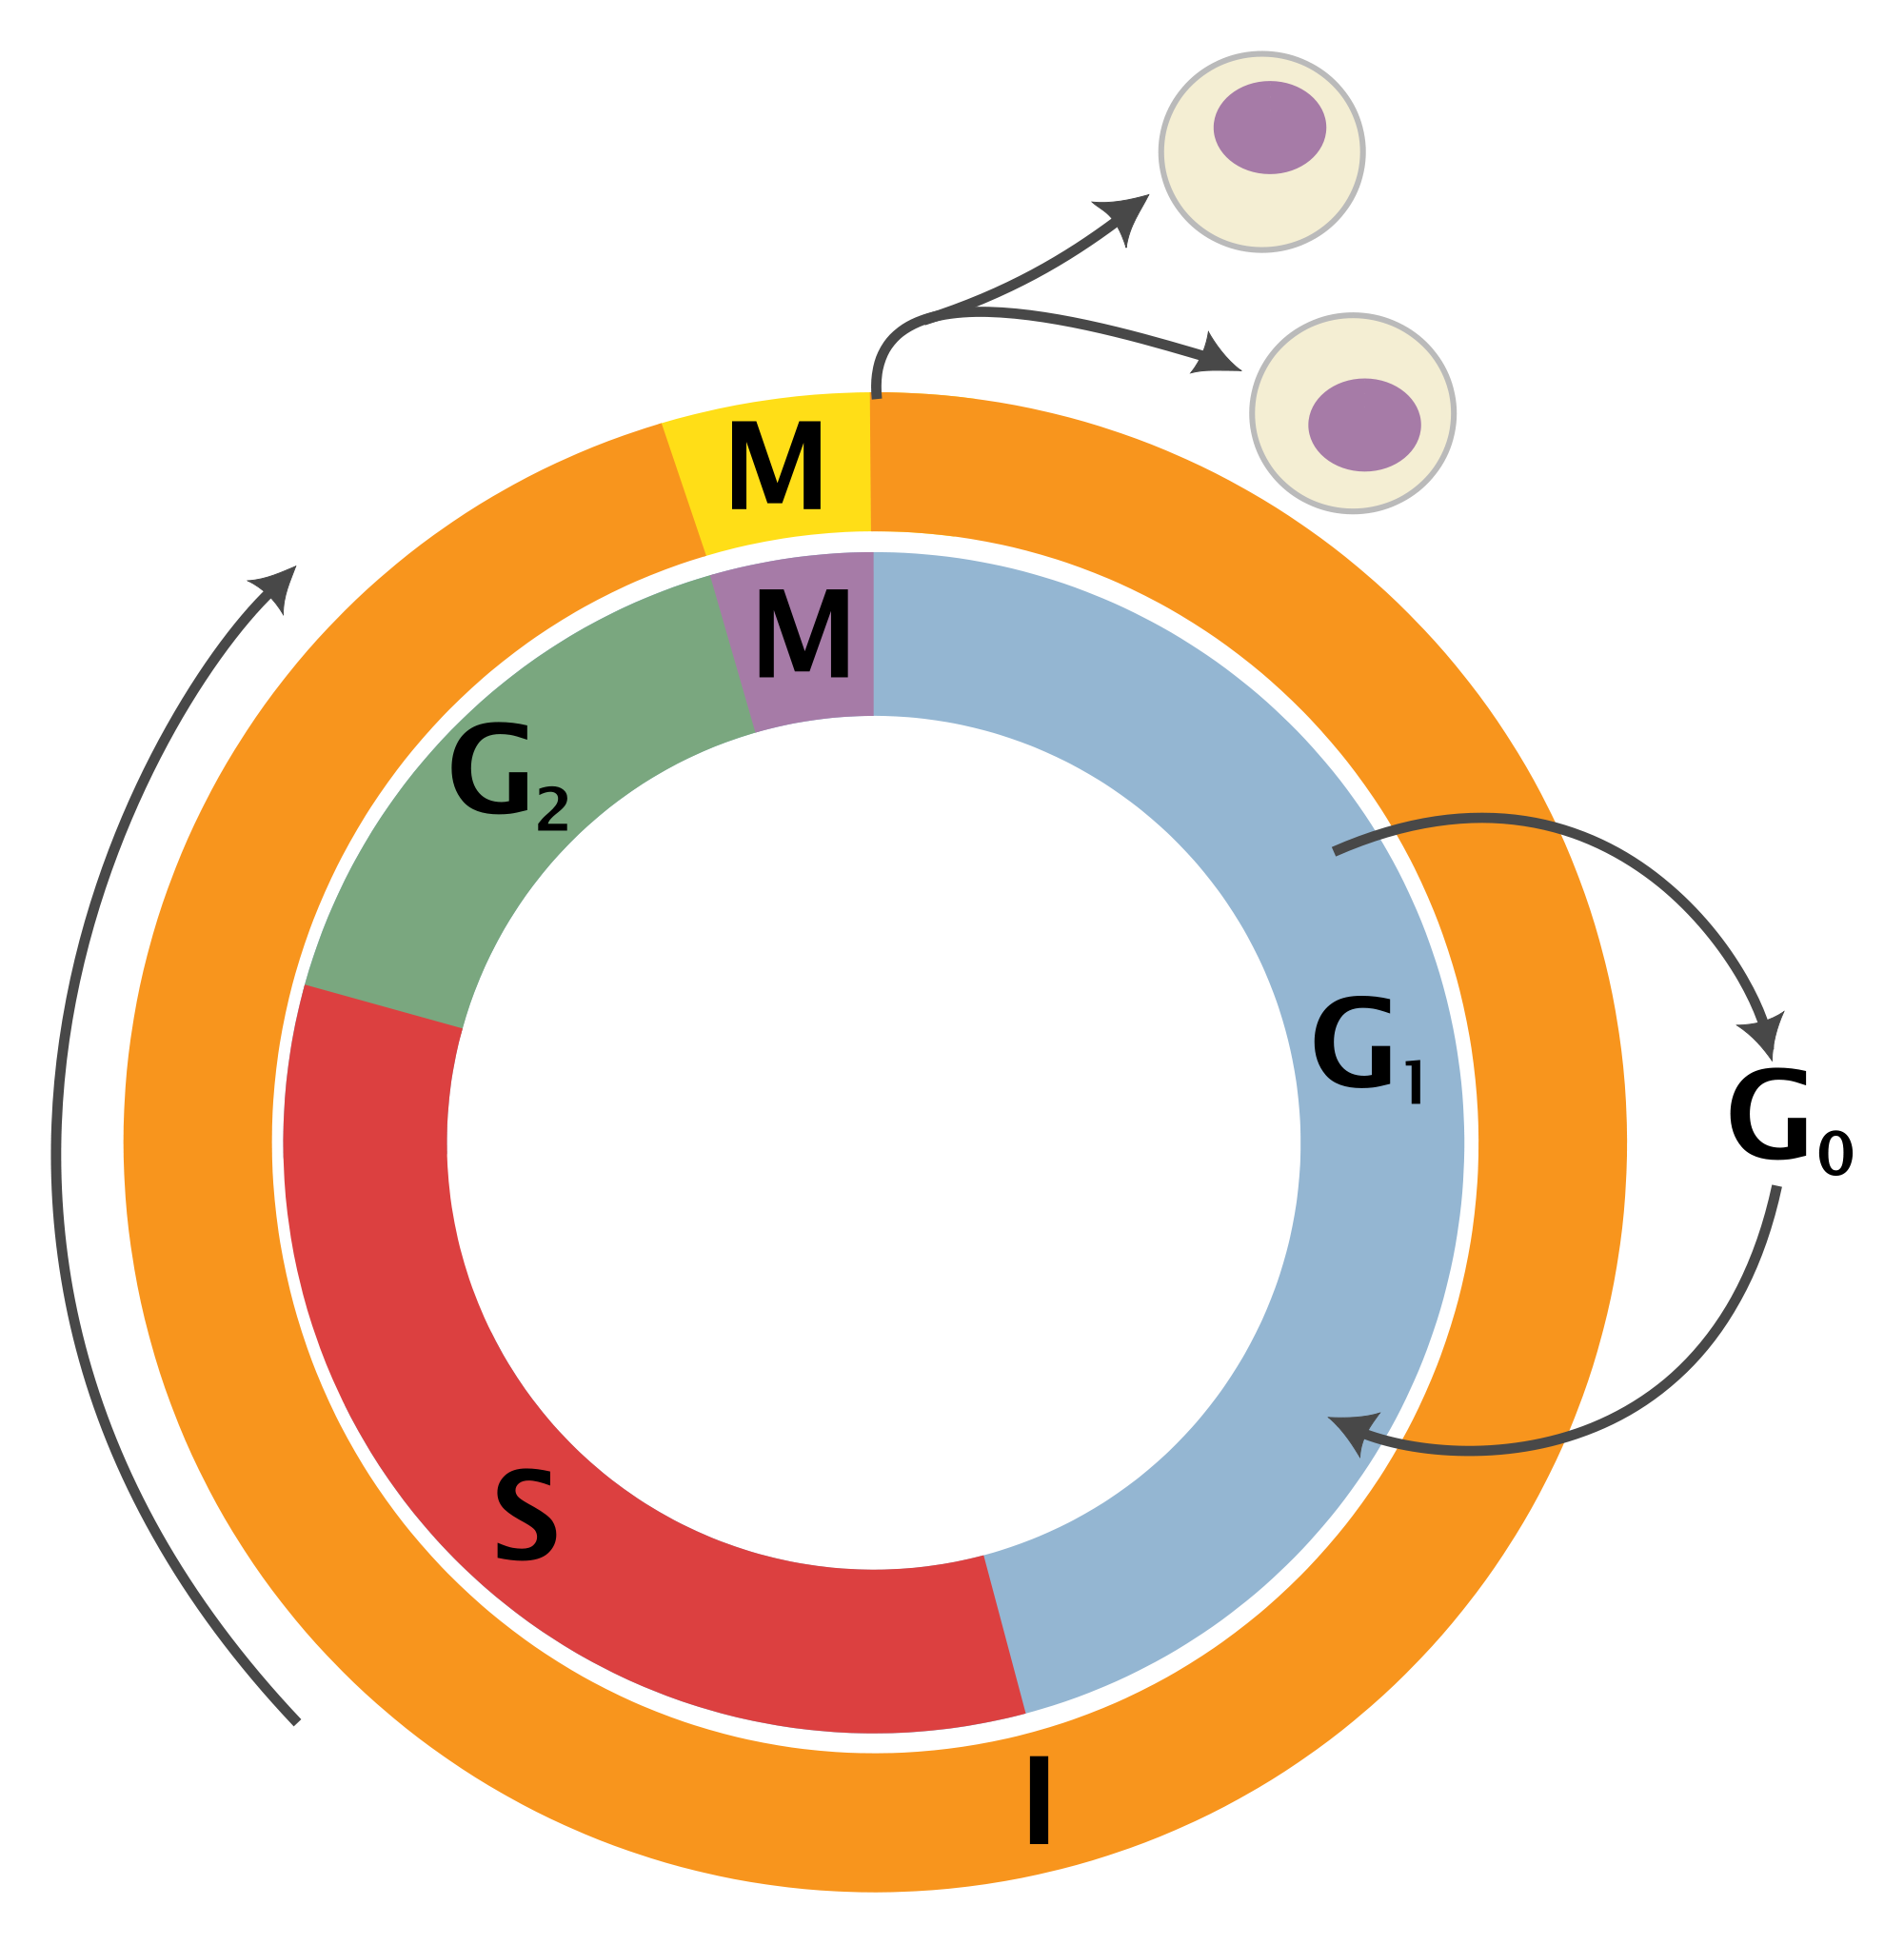
\includegraphics[scale=0.08]{cell_cycle}
\end{center}

In this diagram, the outer ring consists of interphase (labeled $I$), and
mitosis (labeled $M$). The inner ring shows the component parts of interphase
too. The labels are as follows:

\begin{center}
	\begin{tabular}{|c|l|p{5cm}|}

		\hline

		{\bf Label} & {\bf Name} & {\bf Description}\\ \hline

		G1 & Gap phase 1 & Cell grows and new organelles and proteins are
		made.\\ \hline

		S & Synthesis & Cell replicates its DNA, ready to divide by mitosis.\\
		\hline

		G2 & Gap phase 2 & Call keeps growing and proteins needed for division
		are made.\\ \hline

	\end{tabular}
\end{center}

\subsection*{Replication in interphase}

The DNA inside the cell is replicated during interphase. The act of copying the
DNA ensures that each daughter cell has a full set of DNA and he diploid number
of chromosomes is preserved.

The following stages apply to interphase:

\begin{enumerate}

	\item DNA helicase moves along the DNA molecule unzipping it into two single
	strands.

	\item Each original strand acts as a template for a new strand. Nucleotides
	floating in the nucleus join up with their complementary base (A with T, C
	with G). \marginpar{This is called specific base pairing.}

    \item The nucleotdes are joined together at the phosphate backbone by the
	enzyme DNA polymerase. The strands intertwine into a helxical formation 
	again, leaving two identical, yet seperate DNA strands.

\end{enumerate}

This type of replication is called semi-conservative since half of the DNA
strands are conserved and the other half synthesised during replication.

\end{document}